\documentclass[a4paper, 11pt]{article}
\usepackage[UTF8]{ctex}
\usepackage[cpp,table]{mypackage}
\usepackage{cancel,ulem}
\usepackage{amsmath}
\usepackage{graphicx}
\usepackage{geometry}
\usepackage{listings}
\usepackage{forest}
\geometry{scale=0.8}
% \linespread{1.5}
\usepackage[colorlinks,linkcolor=red]{hyperref}

\newcommand{\ent}[4][]{-#1\left(\frac{#2}{#4}\log_2\frac{#2}{#4}+\frac{#3}{#4}\log_2\frac{#3}{#4}\right)}
\newcommand{\ipd}[2]{\partial #1/\partial #2}

\title{
\normalfont \normalsize
\textsc{School of Data and Computer Science, Sun Yat-sen University} \\ [25pt] %textsc small capital letters
\rule{\textwidth}{0.5pt} \\[0.4cm] % Thin top horizontal rule
\huge  T04 Machine Learning\\ % The assignment title
\rule{\textwidth}{2pt} \\[0.5cm] % Thick bottom horizontal rule
\author{17341015 陈鸿峥}
\date{\normalsize\today}
}

\begin{document}
\maketitle
% \tableofcontents

\newpage
\begin{question}\normalfont
Consider the following data. The DECISION-TREE-LEARNING algorithm will first select the attribute \textbf{Length} to split on. Finish building the decision tree, and show the computations.
\begin{center}
\begin{tabular}{|l|l|l|l|l|l|}\hline
    \textbf{Example} & \textbf{Author} & \textbf{Thread} & \textbf{Length} & \textbf{Where Read} & \textbf{User Action (output)}\\\hline
    e1 & known & new & long & home & skips\\\hline
    e2 & unknown & new & short & work & reads\\\hline
    e3 & unknown & follow Up & long & work & skips\\\hline
    e4 & known & follow Up & long & home & skips\\\hline
    e5 & known & new & short & home & reads\\\hline
    e6 & known & follow Up & long & work & skips\\\hline
    e7 & unknown & follow Up & short & work & skips\\\hline
    e8 & unknown & new & short & work & reads\\\hline
    e9 & known & follow Up & long & home & skips\\\hline
    e10 & known & new & long & work & skips\\\hline
    e11 & unknown & follow Up & short & home & skips\\\hline
    e12 & known & new & long & work & skips\\\hline
    e13 & known & follow Up & short & home & reads\\\hline
    e14 & known & new & short & work & reads\\\hline
    e15 & known & new & short & home & reads\\\hline
    e16 & known & follow Up & short & work & reads\\\hline
    e17 & known & new & short & home & reads\\\hline
    e18 & unknown & new & short & work & reads\\\hline
\end{tabular}
\end{center}
\end{question}
\begin{answer}
    按照Length分裂得到如下决策树,其中下划线标识的为reads的标签
\begin{center}
\begin{forest}
[\boxed{\text{Length}}
    [$\substack{1,3,4,6,9,10,12}$,align=center,edge label={node[midway,left,font=\scriptsize]{long}}]
    [$\substack{\underline{2},\underline{5},7,\underline{8},11,\underline{13},\underline{14},\underline{15},\underline{16},\underline{17},\underline{18}}$,align=center,edge label={node[midway,right,font=\scriptsize]{short}}]
]
\end{forest}
\end{center}
    由于左子树全为skips,故不用继续分裂;考虑右子树,分别对剩下的三个属性进行分裂,得到如下决策树
\begin{center}
\begin{forest}
[\boxed{\text{Author}}
    [$\substack{\underline{5},\underline{13},\underline{14},\underline{15},\underline{16},\underline{17}}$,align=center,edge label={node[midway,left,font=\scriptsize]{known}}]
    [$\substack{\underline{2},7,\underline{8},11,\underline{18}}$,align=center,edge label={node[midway,right,font=\scriptsize]{unknown}}]
]
\end{forest}
\qquad
\begin{forest}
[\boxed{\text{Thread}}
    [$\substack{\underline{2},\underline{5},\underline{8},\underline{14},\underline{15},\underline{17},\underline{18}}$,align=center,edge label={node[midway,left,font=\scriptsize]{new}}]
    [$\substack{7,11,\underline{13},\underline{16}}$,align=center,edge label={node[midway,right,font=\scriptsize]{follow Up}}]
]
\end{forest}
\qquad
\begin{forest}
[\boxed{\text{Where Read}}
    [$\substack{\underline{5},11,\underline{13},\underline{15},\underline{17}}$,align=center,edge label={node[midway,left,font=\scriptsize]{home}}]
    [$\substack{\underline{2},7,\underline{8},\underline{14},\underline{16},\underline{18}}$,align=center,edge label={node[midway,right,font=\scriptsize]{work}}]
]
\end{forest}
\end{center}
    分别讨论其信息增益,先计算根节点的信息熵
    \[Ent(D)=\ent{2}{9}{11}=0.684038\]
    然后计算每种划分的信息熵与信息增益
        \[\begin{aligned}
            Gain(D,\text{Author})&=Ent(D)-\sum_{v=1}^2Ent(D^v)\\
            &=Ent(D)-\lrp{\ent[\frac{6}{11}]{6}{0}{6}+\ent[\frac{5}{11}]{3}{2}{5}}\\
            &=0.242697\\
            Gain(D,\text{Thread})&=Ent(D)-\sum_{v=1}^2Ent(D^v)\\
            &=Ent(D)-\lrp{\ent[\frac{7}{11}]{7}{0}{7}+\ent[\frac{4}{11}]{1}{1}{2}}\\
            &=0.320402\\
            Gain(D,\text{Where Read})&=Ent(D)-\sum_{v=1}^2Ent(D^v)\\
            &=Ent(D)-\lrp{\ent[\frac{5}{11}]{4}{1}{5}+\ent[\frac{6}{11}]{1}{5}{6}}\\
            &=0.001331
        \end{aligned}\]
    因此选择Thread进行进一步划分,左子树全为reads,不需划分;只需划分右子树,选择剩下两个属性可以得到
\begin{center}
\begin{forest}
[\boxed{\text{Author}}
    [$\substack{7,11}$,align=center,edge label={node[midway,left,font=\scriptsize]{skips}}]
    [$\substack{\underline{13},\underline{16}}$,align=center,edge label={node[midway,right,font=\scriptsize]{reads}}]
]
\end{forest}
\qquad
\begin{forest}
[\boxed{\text{Where Read}}
    [$\substack{11,\underline{13}}$,align=center,edge label={node[midway,left,font=\scriptsize]{home}}]
    [$\substack{7,\underline{16}}$,align=center,edge label={node[midway,right,font=\scriptsize]{work}}]
]
\end{forest}
\end{center}
    计算根节点的信息熵
    \[Ent(D)=\ent{1}{1}{2}=1\]
    然后计算每种划分的信息熵与信息增益
        \[\begin{aligned}
            Gain(D,\text{Author})&=Ent(D)-\sum_{v=1}^2Ent(D^v)\\
            &=Ent(D)-\lrp{\ent[\frac{1}{2}]{2}{0}{2}+\ent[\frac{1}{2}]{0}{2}{0}}\\
            &=1\\
            Gain(D,\text{Where Read})&=Ent(D)-\sum_{v=1}^2Ent(D^v)\\
            &=Ent(D)-\lrp{\ent[\frac{1}{2}]{1}{1}{2}+\ent[\frac{1}{2}]{1}{1}{2}}\\
            &=0
        \end{aligned}\]
    因而选择Author作为划分属性。
    又划分之后的两个子树内元素均属于同一类别,无法继续划分,决策树算法终止。
    最终得到决策树如下
\begin{center}
\begin{forest}
[\boxed{\text{Length}}
    [$\substack{\text{skips}\\1,3,4,6,9,10,12}$,align=center,edge label={node[midway,left,font=\scriptsize]{long}}]
    [\boxed{\text{Thread}},edge label={node[midway,right,font=\scriptsize]{short}}
        [$\substack{\text{reads}\\2,5,8,14,15,17,18}$,align=center,edge label={node[midway,left,font=\scriptsize]{new}}]
        [\boxed{\text{Author}},edge label={node[midway,right,font=\scriptsize]{follow Up}}
            [$\substack{\text{reads}\\13,16}$,align=center,edge label={node[midway,left,font=\scriptsize]{known}}]
            [$\substack{\text{skips}\\7,11}$,align=center,edge label={node[midway,right,font=\scriptsize]{unknown}}]
        ]
    ]
]
\end{forest}
\end{center}
\end{answer}

\begin{question}\normalfont
Consider the candy example from the lecture. Assume that the prior distribution over $h1, \ldots, h5$ is given by $\lrang{0.1, 0.2, 0.4, 0.2, 0.1}$. Suppose that the first 5 candies taste lime, cherry, cherry, lime, and lime. Make predictions for the 6th candy using Bayesian, MAP and ML learning, respectively. Show
the computations done to make the predictions.
\end{question}
\begin{answer}
    题目中的假设$H$为
    \begin{center}
        \begin{tabular}{|c|c|}\hline
            $h_1$ & 100\% cherry\\\hline
            $h_2$ & 75\% cherry + 25\%  lime\\\hline
            $h_3$ & 50\% cherry + 50\% lime\\\hline
            $h_4$ & 25\% cherry + 75\% lime\\\hline
            $h_5$ & 100\% lime\\\hline
        \end{tabular}
    \end{center}
    给定先验$P(h_i)$和似然$P(d\mid H)$(注意这里假设所有糖果都是独立同分布的)
    \begin{center}
    \begin{tabular}{|c|c|c|c|c|c|}\hline
        hypothesis & $h_1$ & $h_2$ & $h_3$ & $h_4$ & $h_5$\\\hline
        $P(lime\mid h_i)$ & $0$ & $0.25$ & $0.5$ & $0.75$ & $1$\\\hline
        $P(cherry\mid h_i)$ & $1$ & $0.75$ & $0.5$ & $0.25$ & $0$\\\hline
        $P(h_i)$ & $0.1$ & $0.2$ & $0.4$ & 0.2 & $0.1$\\\hline
        $P(d\mid h_i)$ & $(1)^2(0)^3$ & $(0.75)^2(0.25)^3$ & $(0.5)^2(0.5)^3$ & $(0.25)^2(0.75)^3$ & $(0)^2(1)^3$\\
        & $=0$ & $=9/1024$ & $=1/32$ & $=27/1024$ & $=0$\\\hline
    \end{tabular}
    \end{center}
    和证据集
    \[d=\lrang{lime, cherry, cherry, lime, lime}\]
\begin{itemize}
    \item [(a)] 贝叶斯学习:
    由全概率公式
    \[\begin{aligned}
        P(d)&=\sum_i P(d\mid h_i)P(h_i)\\
        &=9/1024\cdot 0.2 + 1/32\cdot 0.4 + 27/1024\cdot 0.2\\
        &=0.01953125
    \end{aligned}\]
    进而
    \[\begin{aligned}
        P(lime \mid d)&=\sum_{i}P(lime\mid h_i)P(h_i\mid d)\\
        &=\frac{1}{P(d)}\sum_iP(lime\mid h_i)P(d\mid h_i)P(h_i)\\
        &=0.01064453125\\
        P(cherry \mid d)&=\sum_{i}P(cherry\mid h_i)P(h_i\mid d)\\
        &=\frac{1}{P(d)}\sum_iP(cherry\mid h_i)P(d\mid h_i)P(h_i)\\
        &=0.00888671875
    \end{aligned}\]
    因$P(lime \mid d)>P(cherry \mid d)$,故判为lime。
    \item [(b)] 极大后验(MAP)
    \[h_{MAP}=\argmax_{h_i} P(h_i\mid d)=\argmax_{h_i} P(h_i)P(d\mid h_i)\]
    可求得
    \[\begin{aligned}
        P(h_1)P(d\mid h_1) &= 0\\
        P(h_2)P(d\mid h_2) &= 0.0017578125\\
        P(h_3)P(d\mid h_3) &= 0.0125\\
        P(h_4)P(d\mid h_4) &= 0.0052734375\\
        P(h_5)P(d\mid h_5) &= 0\\
    \end{aligned}\]
    故$h_{MAP}=h_3$,
    \[\begin{aligned}
        P(lime\mid d)&\approx P(lime\mid h_{MAP})=0.5\\
        P(cherry\mid d)&\approx P(cherry\mid h_{MAP})=0.5
    \end{aligned}\]
    两者预测概率相等。
    \item [(c)] 极大似然(ML)
    \[h_{ML}=\argmax_{h_i} P(d\mid h_i)=h_3\]
    进而
    \[\begin{aligned}
        P(lime\mid d)&\approx P(lime\mid h_{ML})=0.5\\
        P(cherry\mid d)&\approx P(cherry\mid h_{ML})=0.5
    \end{aligned}\]
    两者预测概率相等。
\end{itemize}
\end{answer}

\begin{question}\normalfont
Consider the Boolean function $E = (A\;\mathrm{XOR}\;B) \;\mathrm{AND}\; (C\;\mathrm{XOR}\;D)$. Construct its truth table, and then remove the line for the input $A = 1, B = 1, C = 1, D = 1$. Use Naive Bayes classification to make prediction for this input. Show the computations.
\end{question}
\begin{answer}
真值表如下:
\begin{center}
\begin{longtable}{|c|c|c|c|c|c|}\hline
Sample & A & B & C & D & E\\\hline
1 & 1 & 1 & 1 & 0 & 0\\\hline
2 & 1 & 1 & 0 & 1 & 0\\\hline
3 & 1 & 1 & 0 & 0 & 0\\\hline
4 & 1 & 0 & 1 & 1 & 0\\\hline
5 & 1 & 0 & 1 & 0 & 1\\\hline
6 & 1 & 0 & 0 & 1 & 1\\\hline
7 & 1 & 0 & 0 & 0 & 0\\\hline
8 & 0 & 1 & 1 & 1 & 0\\\hline
9 & 0 & 1 & 1 & 0 & 1\\\hline
10 & 0 & 1 & 0 & 1 & 1\\\hline
11 & 0 & 1 & 0 & 0 & 0\\\hline
12 & 0 & 0 & 1 & 1 & 0\\\hline
13 & 0 & 0 & 1 & 0 & 0\\\hline
14 & 0 & 0 & 0 & 1 & 0\\\hline
15 & 0 & 0 & 0 & 0 & 0\\\hline
\end{longtable}
\end{center}
由朴素贝叶斯
\[\begin{aligned}
P(E\mid A,B,C,D)
&=\frac{P(A,B,C,D\mid E)P(E)}{P(A,B,C,D)}\\
&=\frac{P(A\mid E) P(B\mid E) P(C\mid E) P(D\mid E) P(E)}{P(A,B,C,D)}\\
&=\frac{1/2\cdot 1/2\cdot 1/2\cdot 1/2\cdot 4/15}{1/15}\\
&=\frac{1}{4}\\
P(\lnot E\mid A,B,C,D)
&=\frac{P(A,B,C,D\mid \lnot E)P(\lnot E)}{P(A,B,C,D)}\\
&=\frac{P(A\mid \lnot E) P(B\mid \lnot E) P(C\mid \lnot E) P(D\mid \lnot E) P(\lnot E)}{P(A,B,C,D)}\\
&=\frac{5/11\cdot 5/11\cdot 5/11\cdot 5/11\cdot 11/15}{1/15}\\
&=\frac{625}{1331}
\end{aligned}\]
因为$P(\lnot E\mid A,B,C,D)>P(E\mid A,B,C,D)$,故判别为$E=0$。
\end{answer}

\begin{question}\normalfont
Construct a neural network that computes the $\mathrm{XOR}$ function of two inputs.
\end{question}
\begin{answer}
XOR的真值表如下
\begin{center}
\begin{tabular}{|c|c|c|}\hline
A & B & C\\\hline
0 & 0 & 0\\\hline
0 & 1 & 1\\\hline
1 & 0 & 1\\\hline
1 & 1 & 0\\\hline
\end{tabular}
\end{center}
注意到
\[A \oplus B= (A \lor B) \land (\lnot (A \land B))\]
故可以通过2-2-1的三层神经网络实现,其中输入层对应着$A,B$,隐含层的两个神经元对应着OR和NOT AND的操作,输出层操作则为AND。
进而可构造网络及对应权值如下图所示,其中隐含层及输出层神经元内的数值为偏置(bias)。
\begin{figure}[H]
\centering
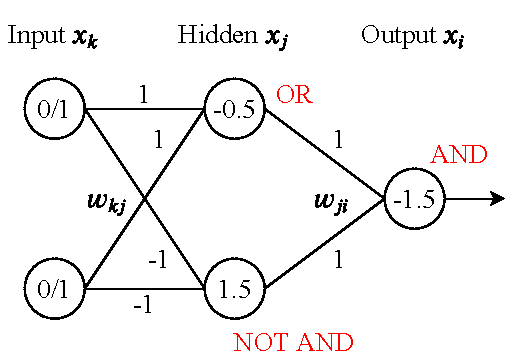
\includegraphics[width=0.5\linewidth]{fig/T04-Q4.pdf}
\end{figure}
并且令隐含层和输出层的激活函数都为
\[\sigma(x)=\begin{cases}
    1 & x > 0\\
    0 & x\leq 0
\end{cases}\]
则前向传播规则为
\[f(x_1,x_2)=x_i=\sigma\left(\sum_j w_{ji}\sigma\left(\sum_k w_{kj}x_k + b_j\right)+b_i\right)\]
进而
\[\begin{aligned}
    f(0,0)&=\sigma(\sigma(0*1+0*1-0.5)*1+\sigma(0*(-1)+0*(-1)+1.5)*1-1.5)=\sigma(0+1-1.5)=0\\
    f(0,1)&=\sigma(\sigma(0*1+1*1-0.5)*1+\sigma(0*(-1)+1*(-1)+1.5)*1-1.5)=\sigma(1+1-1.5)=1\\
    f(1,0)&=\sigma(\sigma(1*1+0*1-0.5)*1+\sigma(1*(-1)+0*(-1)+1.5)*1-1.5)=\sigma(1+1-1.5)=1\\
    f(1,1)&=\sigma(\sigma(1*1+1*1-0.5)*1+\sigma(1*(-1)+1*(-1)+1.5)*1-1.5)=\sigma(1+0-1.5)=0
\end{aligned}\]
即为所求的XOR网络。
\end{answer}

\begin{question}\normalfont
Consider the neural net on Page 32 of the course slides for neural nets.
\begin{figure}
\centering
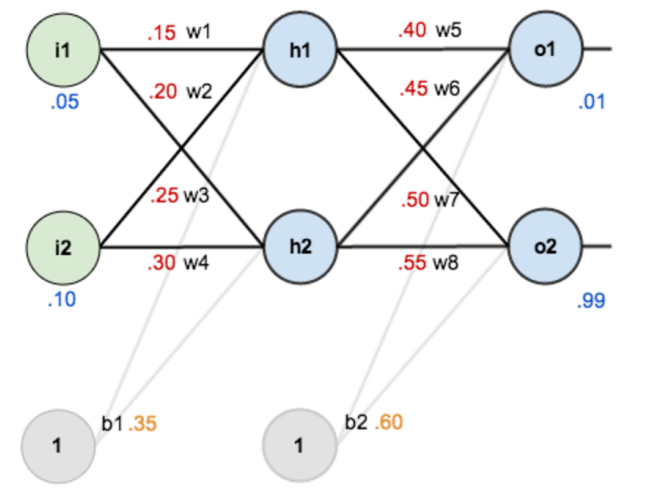
\includegraphics[width=0.5\linewidth]{fig/neural_net.png}
\end{figure}
\begin{itemize}
\item[(a)] Suppose we use the sigmoid function as the activate function. Compute $\pd{Loss_{o1}}{w_1}$.
\item[(b)] Suppose we use the $\tanh$ function as the activate function. Compute $\pd{Loss_{o2}}{w_4}$. Note that
\[\begin{aligned}
    \tanh(x) &= (\ee^x - \ee^{-x})/(\ee^x + \ee^{-x}) = 2g(2x) - 1\\
    \tanh'(x) &= 1 - \tanh^2(x)
\end{aligned}\]
\end{itemize}
\end{question}
% https://mattmazur.com/2015/03/17/a-step-by-step-backpropagation-example/
\begin{answer}
    这里损失函数采用平方误差
    \[Loss=\sum_{k}Loss_k\qquad Loss_k=(y_k-a_k)^2\]
\begin{itemize}
    \item[(a)] 先计算前向过程
    \[\begin{array}{llll}
        in_{h1} &= w_1 i_1 + w_2 i_2 + b_1 &= 0.05\cdot 0.15 + 0.10 \cdot 0.20 + 0.35 &= 0.3775\\
        in_{h2} &= w_3 i_1 + w_4 i_2 + b_1 &= 0.05\cdot 0.25 + 0.10 \cdot 0.30 + 0.35 &= 0.3925\\
        out_{h1} &= g(in_{h1}) &= \frac{1}{1+\ee^{-0.3775}} &=0.593269992\\
        out_{h2} &= g(in_{h2}) &= \frac{1}{1+\ee^{-0.3875}} &=0.596884378\\
        in_{o1} &= w_5 out_{h1} + w_6 out_{h2} +b_2 &= 0.4\cdot 0.59326992 + 0.45\cdot 0.596884378 + 0.60 &= 1.1059059669\\
        in_{o2} &= w_7 out_{h1} + w_8 out_{h2} +b_2 &= 0.5\cdot 0.59326992 + 0.55\cdot 0.596884378 + 0.60 &= 0.909921369\\
        out_{o1} &= g(in_{o1}) &=\frac{1}{1+\ee^{-1.1059059669}} &= 0.751365070\\
        out_{o2} &= g(in_{o2}) &=\frac{1}{1+\ee^{-0.909921369}} &= 0.772928459\\
        Loss_{o1} &= (target_{o1}-out_{o1})^2 &= (0.01-0.751365070)^2 &=0.5496221670\\
        Loss_{o2} &= (target_{o2}-out_{o2})^2 &= (0.99-0.772928459)^2 &=0.0471200539
    \end{array}\]
    再计算后向梯度
    \[\pd{Loss_{o1}}{w_1}=\pd{Loss_{o1}}{out_{o1}}\pd{out_{o1}}{in_{o1}}\pd{in_{o1}}{out_{h1}}\pd{out_{h1}}{in_{h1}}\pd{in_{h1}}{w_1}\]
    \[\begin{array}{lll}
        \ipd{Loss_{o1}}{out_{o1}}&=2(target_{o1}-out_{o1})&=-1.48273014\\
        \ipd{out_{o1}}{in_{o1}}&=out_{o1}(1-out_{o1})&=0.1868156\\
        \ipd{in_{o1}}{out_{h1}}&=w_5&=0.40\\
        \ipd{out_{h1}}{in_{h1}}&=out_{h1}(1-out_{h1})&=0.24130071\\
        \ipd{in_{h1}}{w_1}&=i1&=0.05
    \end{array}\]
    进而
    \[\pd{Loss_{o1}}{w_1}=-0.00133679\]
    \item[(b)] 先计算前向过程
    \[\begin{array}{lll}
        in_{h1} &= w_1 i_1 + w_2 i_2 + b_1 &= 0.3775\\
        in_{h2} &= w_3 i_1 + w_4 i_2 + b_1 &= 0.3925\\
        out_{h1} &= \tanh(in_{h1}) &=0.36053439\\
        out_{h2} &= \tanh(in_{h2}) &=0.37351345\\
        in_{o1} &= w_5 out_{h1} + w_6 out_{h2} +b_2 &= 0.912312211\\
        in_{o2} &= w_7 out_{h1} + w_8 out_{h2} +b_2 &= 0.985721346\\
        out_{o1} &= \tanh(in_{o1}) &= 0.722240193\\
        out_{o2} &= \tanh(in_{o2}) &= 0.755531976\\
        Loss_{o1} &= (target_{o1}-out_{o1})^2 &=0.50728609\\
        Loss_{o2} &= (target_{o1}-out_{o2})^2 &=0.05497525
    \end{array}\]
    再计算后向梯度
    \[\pd{Loss_{o2}}{w_4}=\pd{Loss_{o2}}{out_{o2}}\pd{out_{o2}}{in_{o2}}\pd{in_{o2}}{out_{h2}}\pd{out_{h2}}{in_{h2}}\pd{in_{h2}}{w_4}\]
    \[\begin{array}{llll}
        \ipd{Loss_{o2}}{out_{o2}}&=2(target_{o2}-out_{o2})&=0.468936048\\
        \ipd{out_{o2}}{in_{o2}}&=1-out_{o2}^2&=0.429171433\\
        \ipd{in_{o2}}{out_{h2}}&=w_8&=0.55\\
        \ipd{out_{h2}}{in_{h2}}&=1-out_{h2}^2&=0.8604877\\
        \ipd{in_{h2}}{w_4}&=i2&=0.10
    \end{array}\]
    进而
    \[\pd{Loss_{o2}}{w_4}=0.009524710\]
\end{itemize}
\end{answer}

\end{document}